% Unofficial UofT Statistical Sciences Poster template.
% A fork of the UMich template https://www.overleaf.com/latex/templates/university-of-michigan-umich-poster-template/xpnqzzxwbjzc
% which is fork of the MSU template https://www.overleaf.com/latex/templates/an-unofficial-poster-template-for-michigan-state-university/wnymbgpxnnwd
% which is a fork of https://www.overleaf.com/latex/templates/an-unofficial-poster-template-for-new-york-university/krgqtqmzdqhg
% which is a fork of https://github.com/anishathalye/gemini
% also refer to https://github.com/k4rtik/uchicago-poster

\documentclass[final]{beamer}

% ====================
% Packages
% ====================
\usepackage{graphicx}
\usepackage{subcaption}
\usepackage[T1]{fontenc}
 \usepackage[utf8]{luainputenc}
\usepackage{lmodern}
\usepackage[size=custom, width=122,height=91, scale=1.2]{beamerposter}
\usepackage{fontspec}
\usetheme{gemini}
\usecolortheme{uoft}
\usepackage{graphicx}
\usepackage{booktabs}
\usepackage{tikz}
\usepackage{pgfplots}
\pgfplotsset{compat=1.14}
\usepackage{anyfontsize}


\usepackage{amsmath}
\DeclareMathOperator*{\argmax}{arg\,max}
\DeclareMathOperator*{\argmin}{arg\,min}
\DeclareMathOperator{\proj}{proj}
\usepackage{comment}
\usepackage{multicol}



% ====================
% Lengths
% ====================

% If you have N columns, choose \sepwidth and \colwidth such that
% (N+1)*\sepwidth + N*\colwidth = \paperwidth
\newlength{\sepwidth}
\newlength{\colwidth}
\setlength{\sepwidth}{0.025\paperwidth}
\setlength{\colwidth}{0.3\paperwidth}

\newcommand{\separatorcolumn}{\begin{column}{\sepwidth}\end{column}}

% ====================
% Title
% ====================

\title{Monotone Density Estimation with Wasserstein Projection}

\author{Lessard, Charles-Étienne; Liu, Zirui; Shen, Ruihang; Shirani, Parsa\\Supervised by Wong, Leonard; Gunasingam, Madhu}

\institute[shortinst]{Department of Statistical Sciences, University of Toronto}

% ====================
% Footer (optional)
% ====================

\footercontent{
  \href{https://www.statistics.utoronto.ca/}{StatSci: https://www.statistics.utoronto.ca} \hfill
  \href{mailto:youremail@utoronto.ca}{youremail@utoronto.ca}}
% (can be left out to remove footer)

% ====================
% Logo (optional)
% ====================

% use this to include logos on the left and/or right side of the header:
% Left: institution
 \logoright{
\includegraphics[height=8cm]{logos/logo.png}}
 \logoleft{
\includegraphics[height=8cm]{logos/logo.png}}
% Right: funding agencies and other affiliations 
%\logoright{\includegraphics[height=7cm]{logos/NSF.eps}}
% ====================
% Body
% ====================

\begin{document}



\begin{frame}[t]
\begin{columns}[t]
\separatorcolumn

\begin{column}{\colwidth}

  \begin{block}{Abstract}

    This project investigated a novel approach to nonparametric density estimation under a monotonicity constraint, using optimal transport theory. While the Grenander estimator offers a classical solution by maximizing likelihood over non-increasing densities on $\mathbb{R}_+$, this project proposed an alternative method based on projecting the empirical distribution onto a convex set of probability measures whose quantile functions are convex and anchored at zero. This allows reformulation as a 2-Wasserstein projection in a Hilbert space, enabling efficient computation via convex optimization. This project implemented Wasserstein estimator, evaluated its performance via simulations. The project also analyzed its rate of convergence in comparison with the Grenander estimator, and proved the Wasserstein estimator is consistent.

    %\begin{figure}
     
     %\centering
      %              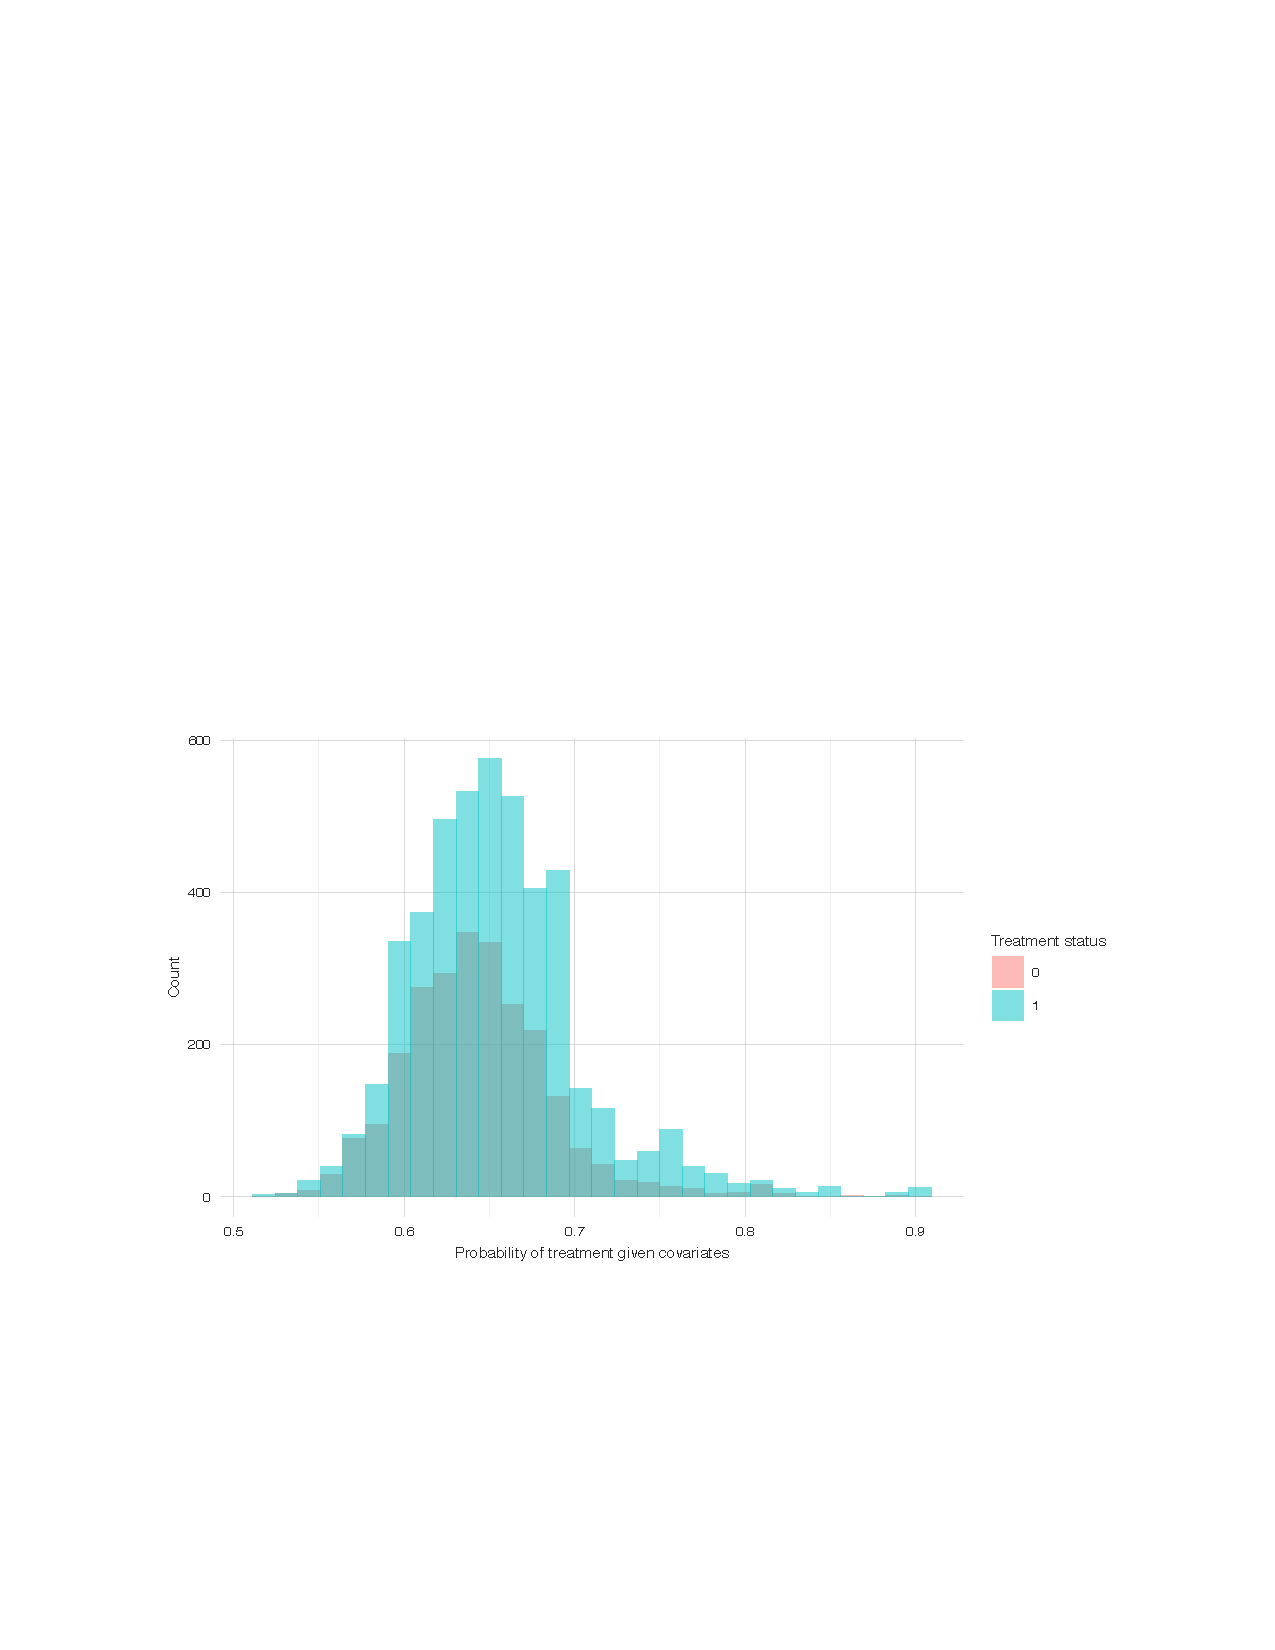
\includegraphics[width=0.6\textwidth]{figures/results_fig.pdf}
    %\end{figure}

  
  \end{block}

  


  \begin{block}{Setting}

  In this project we consider i.i.d.~samples from a density $f$ on $\mathbb{R}_+$ such that: 
    \begin{itemize}
    %\item $X_i \geq 0$ are i.i.d.~samples from a density $f$
    \item $f$ is non-increasing on $\mathbb{R}_+$: for all $x \leq y$, we have $f(x) \geq f(y)$.% on $[0;\infty)$.
    \item $f$ has a finite second moment: $\int_0^\infty x^2 f(x)\, dx < \infty$.
  \end{itemize}
  We let $\mathcal{F}_0$ be the set of all such densities. Given observations $x_1,x_2,...,x_n > 0$, we say $\hat{f}$ is the \textbf{Grenander estimator} with respect to $\mathcal{F}_0$ if \begin{equation*} %\label{eqn:MLE}
\hat{f} \in \argmax_{f \in \mathcal{F}_0} \sum_{i = 1}^n \log f(x_i).
\end{equation*}

If $\mu$ is a probability distribution, we let $ Q_{\mu}(u) = \inf\{ x : F_{\mu}(x) \geq u \}$ be its quantile function. For any probability distributions $\mu,\nu$, we define the \textbf{$2$-Wasserstein distance} $\mathcal{W}_2(\mu, \nu)$ by the $L^2$ distance between their quantile functions: 
\begin{equation*}
\mathcal{W}_2(\mu, \nu) = \| Q_{\mu} - Q_{\nu} \|_{L^2([0, 1])}.
\end{equation*}

Let $\mathcal{F}$ be a set of distributions $\mu$ on $\mathbb{R}_+$ such that their quantile functions $Q_{\mu}$ satisfy:
\vspace{-1.5cm}
\begin{itemize}
\item[(i)] $Q_{\mu}$ is non-decreasing.
\item[(ii)] $Q_{\mu}(0) = \lim_{u \rightarrow 0^+} Q_{\mu}(u) = 0$.
\item[(iii)] $Q_{\mu}$ is convex.
\end{itemize}
It can be shown that $\mathcal{F}$ is the $\mathcal{W}_2$-closure of $\mathcal{F}_0$. Define $\mathcal{Q} = \{Q_{\mu} : \mu \in \mathcal{F}\}$ as the set of quantile functions of distributions in $\mathcal{F}$. \\
\vspace{1cm}
\textbf{(Wasserstein Projection)}: For $\mu \in \mathcal{P}_2(\mathbb{R}_+)$, there exists unique $\mu^* \in \mathcal{F}$ such that 
\begin{equation*} %\label{eqn:Wasserstein.projection},
\mu^* = \argmin_{\nu \in \mathcal{F}} \mathcal{W}_2(\nu, \mu). 
\end{equation*}
We write $\mu^* = \proj_{\mathcal{F}} \mu$. This is equivalent to finding
\begin{equation*}
Q^* = \min_{Q \in \mathcal{Q}} \| Q - Q_{\mu} \|_{L^2([0, 1])}^2.
\end{equation*}

(\textbf{Wasserstein Density Estimator}): Given data points $x_1, \ldots, x_n > 0$, consider the empirical distribution $\mu_n = \sum_{i = 1}^n \frac{1}{n} \delta_{x_i}$. The Wasserstein density estimator $\hat{\mu}_n$ with respect to $\mathcal{F}$ is defined by the Wasserstein projection onto $\mathcal{F}$:\\
\vspace{1cm}
\centering$\hat{\mu}_n = \proj_{\mathcal{F}} \mu_n$ with quantile function $Q_{\hat{\mu}_n} = \min_{Q \in \mathcal{Q}} \| Q - Q_{\hat{\mu}_n}\|_{L^2([0, 1])}^2$. 





%\begin{itemize}
%\item \textbf{Implementation:} To implement the Wasserstein estimator for density estimation.
%\item \textbf{Empirical and Power Law Evaluation:} To evaluate the Wasserstein estimator's empirical and power law performance via simulations
%\item \textbf{Comparison and Analysis:} To compare the Wasserstein estimator with the Grenander estimator, and to analyze their convergence properties.
%\item \textbf{Theoretical Properties:} To prove the Wasserstein estimator is consistent.
%\end{itemize}

\end{block}



\end{column}

\separatorcolumn

\begin{column}{\colwidth}
\begin{alertblock}{Implementation}
    \begin{itemize}
        \item \textbf{Wasserstein density estimator:} We implemented the Wasserstein density estimator in three steps:
\begin{enumerate}
  \item \textbf{Empirical quantile.} On the uniform grid
    $0 = u_0 < u_1 < \cdots < u_n = 1$, compute the empirical quantile function $Q_{\rm emp}$ based on the data.
%    \[
%      Q_{\rm emp}(u_j)
%      =
%      \text{interp}\Bigl(\tfrac{1}{n},\tfrac{2}{n},\dots,1;
%                x_{(1)},x_{(2)},\dots,x_{(n)};\; u_j\Bigr),
%    \]
%    by sorting the sample \(x_{(1)}\le\cdots\le x_{(n)}\) and linearly
 %   interpolating.
  \item \textbf{Projection via quadratic programming.} Using the \texttt{cvxpy} package in Python, solve
    \[
      \min_{Q\in\mathbb{R}^n}
        \frac{1}{n}\sum_{j=0}^n \bigl(Q_j - Q_{\rm emp}(u_j)\bigr)^2
    \]
    subject to $Q_0 = 0$, $Q_j \leq Q_{j+1}$ (monotonicity), and $Q_{j+2} - 2\,Q_{j+1} + Q_j \ge 0$ (convexity) to obtain \(Q^*\).
  \item \textbf{Density recovery.} Invert the projected quantile
    \(Q^*\) to get an approximate cumulative distribution function and hence the density.
\end{enumerate}
\item \textbf{Grenander estimator:} We used the R package \texttt{fdrtool}.

\end{itemize}
   \end{alertblock}
\begin{block}{Findings}

\centering

\vspace{0.1em}

% --- Second Image ---

\begin{subfigure}[b]{0.45\textwidth}
  \centering
  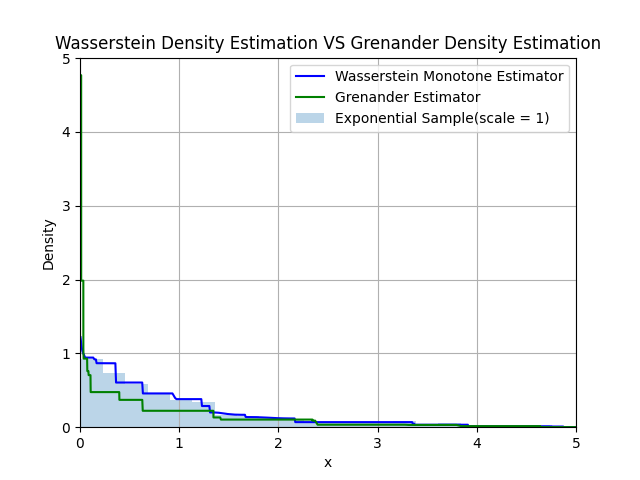
\includegraphics[width=\textwidth]{UofT Poster Template Tex/figures/WDE VS GDE.png}
  {\small\textit{Figure 1: Wasserstein Estimator and Grenander Estimator estimating the exponential distribution}}

\end{subfigure}
\hfill
\begin{subfigure}[b]{0.5\textwidth}
  \centering
  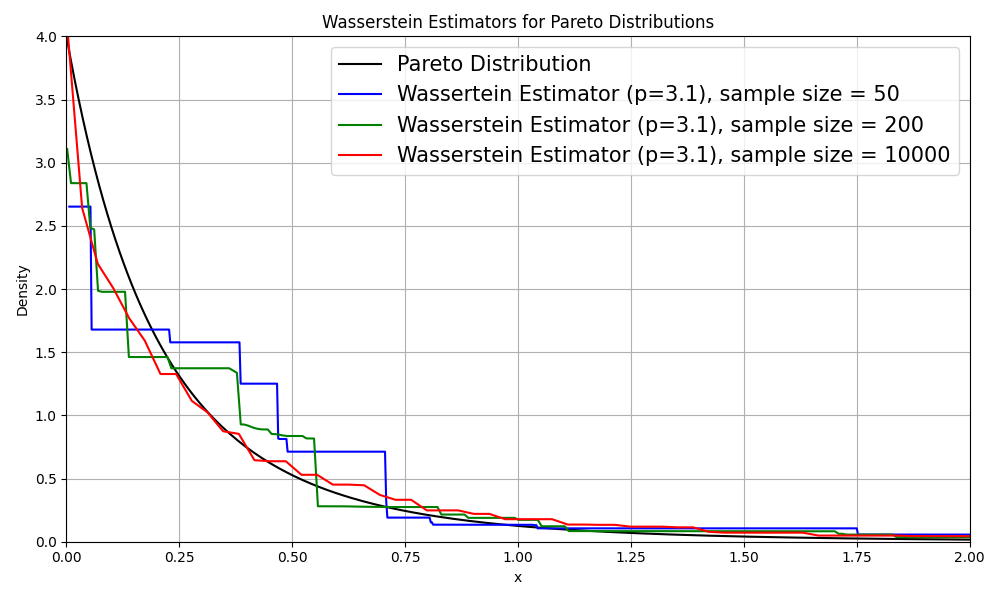
\includegraphics[width=\textwidth]{UofT Poster Template Tex/figures/Pareto_distributions.png}
  \small\textit{Figure 2: Wasserstein Estimator using different sample sizes estimating the Pareto distribution}
\end{subfigure}

\vspace{0.1em}



\vspace{2cm}

% --- Subfigures (p = 3.1, 5, 10) ---
\centering
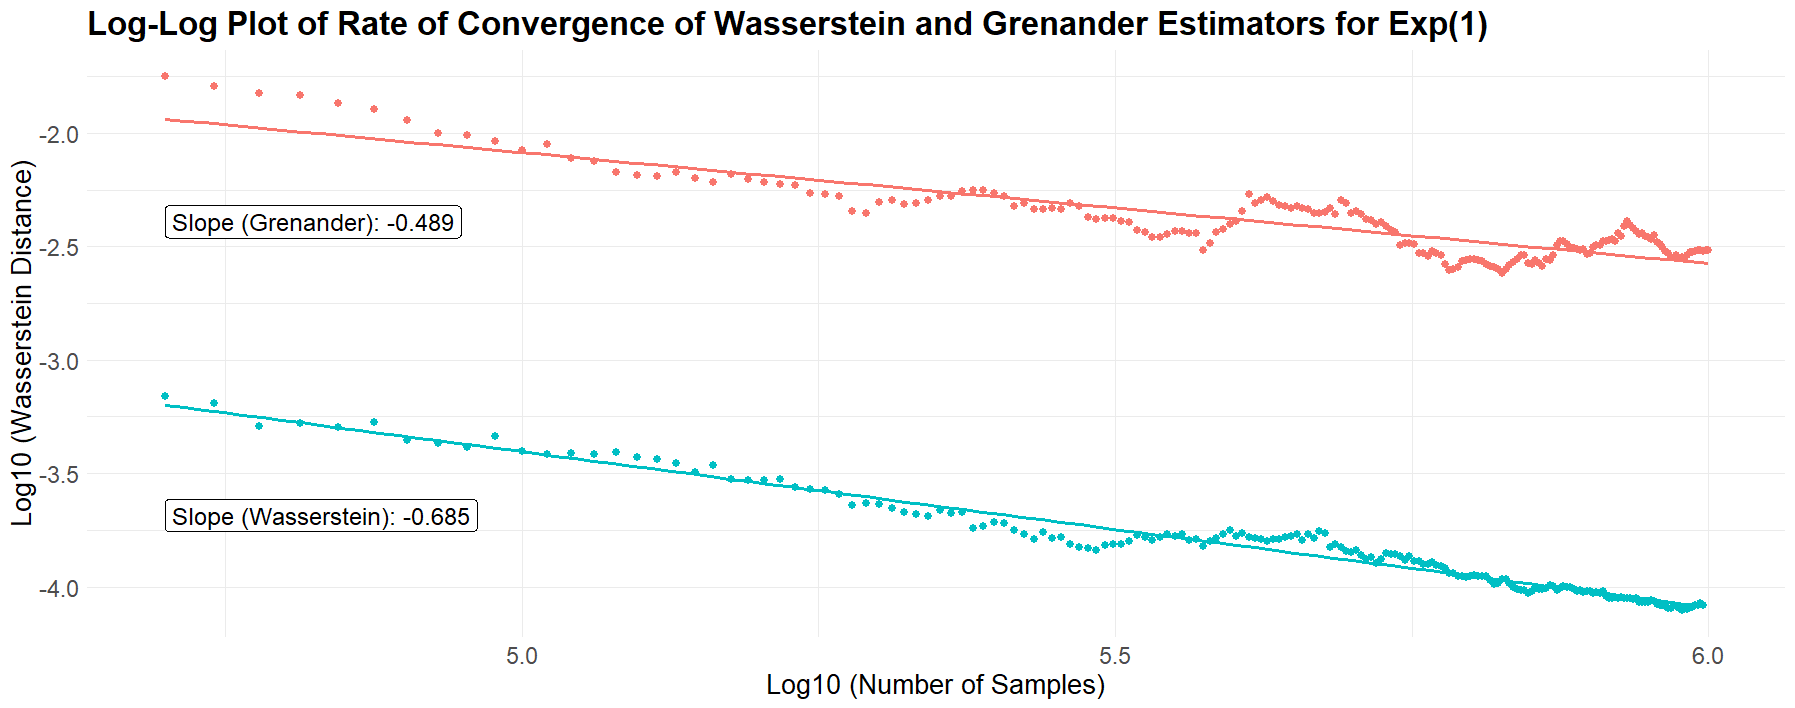
\includegraphics[width=1\textwidth, height=20cm]{UofT Poster Template Tex/figures/Plot_Data2.png}
\vspace{0.1em}
\textit{Figure 3: Log-log plot comparison between Wasserstein and Grenander Density Estimators estimating the exponential distribution (rate = 1)}

\vspace{0.1em}



\end{block}



\end{column}

\separatorcolumn

\begin{column}{\colwidth}

  \begin{exampleblock}{Theoretical properties of the Wasserstein density estimator}

\noindent\textbf{Theorem:} The Wasserstein density estimator is consistent.\\[0.5em]
\[
\mathcal{W}_2(\hat{\mu}_n, \mu^*) \xrightarrow{a.s.} 0
\]\\[0.5em]

\noindent\textbf{Proof:}\, 
Observe that \[
\mathcal{W}_2(\hat{\mu}_n, \mu^*) = \mathcal{W}_2\left( \mathrm{proj}_{\mathcal{F}}(\mu_n), \mathrm{proj}_{\mathcal{F}}(\mu) \right) \leq \mathcal{W}_2(\mu_n, \mu) \hspace{2em} (1)
\] by 1-Lipschitz continuity of the projection operator. Since the empirical measure is $\mathcal{W}_2$-consistent we have $\mathcal{W}_2(\mu_n, \mu) \xrightarrow{a.s.} 0$ and thus $\mathcal{W}_2(\hat{\mu}_n, \mu^*) \xrightarrow{a.s.} 0$ as desired.\vspace{1cm}
\noindent\textbf{Theorem:} Suppose $\mu^*$ is log-concave, then there exists $C > 0$ such that\\[0.5em]
\[
\mathbb{E}\left[ \mathcal{W}_2^2(\hat{\mu}_n, \mu^*) \right] \leq \frac{C  \log n}{n}.
\]
\noindent\textbf{Proof:}\, 
From (1), we have 
\[
\mathbb{E}\left[ \mathcal{W}_2^2(\hat{\mu}_n, \mu^*) \right] \leq \mathbb{E}\left[ \mathcal{W}_2^2(\mu_n, \mu) \right].
\]
And by [1], $\mathbb{E}\left[ \mathcal{W}_2^2(\mu_n, \mu) \right] \leq \frac{C \log n}{n}$, where $C = C'\sigma^2$ with $\sigma^2$ the variance of $\mu$ and $C' > 0$.




\end{exampleblock}

  \begin{block}{Conclusions}

     On the exponential distribution with rate 1, we observe that:
     \begin{itemize}
         \item The Wasserstein distance of the Wasserstein estimator is significantly smaller than the Wasserstein distance of the Grenander estimator.
         \item The Wasserstein estimator converges faster than the Grenander estimator.
     \end{itemize}
     
     The Wasserstein estimator also demonstrates strong empirical performance on other distribution families, including the Pareto distribution. Finally, it possesses strong theoretical properties such as consistency and rapid convergence in expectation. 
     %Finally, we proved that the %Wasserstein density estimator is %consistent.

    %\begin{table}
      %\centering
      %\begin{tabular}{l r r c}
        %\toprule
        %\textbf{First column} & \textbf{Second column} & \textbf{Third column} & \textbf{Fourth} \\
        %\midrule
        %Chicken & 13.37 & 384,394 & $\alpha$ \\
        %Hen & 2.17 & 1,392 & $\beta$ \\
       % Rooster & 3.14 & 83,742 & $\delta$ \\
        %Egg & 7.59 & 974 & $\gamma$ \\
        %\bottomrule
      %\end{tabular}
      %\caption{A table caption.}
   % \end{table}
  \end{block}

  \begin{block}{References}

    \nocite{*}
    \footnotesize{\bibliographystyle{plain}}
    \bibliography{references_poster} 

  \end{block}

  \begin{block}{Contact}
  \textbf{Charles-Étienne Lessard}: charles-etienne.lessard@mail.mcgill.ca \\
  \textbf{Zirui Liu}: rayxxx.liu@mail.utoronto.ca\\
  \textbf{Ruihang Shen}: ruihang.shen@mail.mcgill.ca\\
  \textbf{Parsa Shirani}: parsa.shirani@mail.mcgill.ca \\ 
  
      
  \end{block}

\end{column}

\separatorcolumn
\end{columns}
\end{frame}

\end{document}
